\documentclass[12pt, oneside]{article}
\usepackage{geometry}
\geometry{letterpaper}
\usepackage{graphicx}
\graphicspath{{images/}}
\usepackage{amsmath}
\usepackage{amsthm}
\usepackage{amssymb}
\usepackage{diagbox}
\usepackage{mathtools}
\usepackage{hyperref}
\usepackage{tikz}
\usetikzlibrary {shapes.geometric}
\usetikzlibrary{angles,quotes}
\hypersetup{
	colorlinks=true,
	urlcolor=blue
}

\title{Math Journal}
\author{Andrew Ha}
\date{}								%no date

\newtheorem{proposition}{Proposition}
\newtheorem{identity}{Identity}

\begin{document}
\maketitle
\section*{Combinatorial Proof}
\textbf{09/10/2024}
\begin{proposition} For positive integers $n$ and $k$ with $n=2k, \frac{n!}{2!^k}$ is an integer. \end{proposition}
\emph{Proof.}  Consider the $n$ symbols: $x_1, x_1, x_2, x_2, \cdots, x_k, x_k$.
The number of arrangements of all these $n = 2k$ symbols is an integer that equals
\[
\frac{n!}{\underbrace{2! 2! \cdots 2!}_{\text{k factors of 2!}}} = \frac{n!}{2!^k}
\]
I learned this from the first day of class in MACM 101. This is an example of proving that a value is an integer by obtaining that value from counting something. Researching further, I also found out about double counting.\ It is based on the idea that counting the same objects in two different ways results in two different expressions, which must be equal to each other. 
\begin{identity}
\[
2^n = \sum_{k=0}^{n}  \binom{n}{k}
\]
\end{identity}
For example, this identity can be proved by counting the number of subsets of a set $A$ with $n$ elements. One way to count this is noticing how you can either include or exclude each element, giving 2 choices for each of the $n$ elements. This gives $2^n$ subsets. Second way to count the number of subsets is summing up the number of subsets with $k$ elements where $k$ can be any integer from 0 to $n$. For each case, you would be choosing $k$ elements out of $n$ elements, so there are $\binom{n}{k}$ subsets.
Summing up, the total number of subsets is $\sum_{k=0}^{n}  \binom{n}{k}$.\ Two expressions, $2^n$ and $\sum_{k=0}^{n}  \binom{n}{k}$, must be equal since they represent the same thing.
\section*{Putnam 2002 B1}
\textbf{09/11/2024}
\\
\noindent Here is a fun problem I wanted to share from the 2002 William Lowell Putnam Mathematics Competition.
\begin{quote}
B1. Shanille O'Keal shoots free throws on a basketball court. She hits
the first and misses the second, and thereafter the probability that
she hits the next shot is equal to the proportion of shots she
has hit so far. What is the probability she hits exactly 50 of
her first 100 shots?
\end{quote}
This problem doesn't require much of advanced mathematics, yet it is simple and tricky. Here's a solution I like:\\

\emph{Solution.} The probability of $n$th success is the proportion of shots she has hit so far, which is $\frac{n - 1}{\text{\# of shots so far}}$. On the other hand, the probability of $n$th miss is $1 - \frac{\text{\# of successes so far}}{\text{\# of shots so far}} = \frac{\text{\# of shots so far}}{\text{\# of shots so far}} - \frac{\text{\# of shots so far} - (n - 1)}{\text{\# of shots so far}} = \frac{n-1}{\text{\# of shots so far}}$. For her to hit exactly 50 of her first 100 shots, she has to hit exactly 49 shots and miss exactly 49 shots. Consider the probability of one case where she hits 49 shots consecutively then misses 49 shots consecutively: 
\[
\underbrace{\frac{1}{2} \times \frac{2}{3} \times \frac{3}{4} \times \frac{4}{5} \times \cdots \times \frac{49}{50}}_\text{49 successes} \times \underbrace{\frac{1}{51} \times \frac{2}{52} \times \frac{3}{53} \times \frac{4}{54} \cdots \times \frac{49}{99}}_\text{49 misses} = \frac{49!^2}{99!}
\]
Here, the arrangement of shots does not affect the overall probability since the numerator will always be $49!^2$ as long as she hits 49 shots and misses 49 shots, and the denominator will always be 99!. Therefore, multiplying the probability of single case by the number of arrangements will give us the answer. The number of arrangements of 49 shots and 49 misses is $\frac{98!}{49!^2}$ since there are 49 duplicates of 2 cases. Multiplying two numbers yields
\[
\frac{49!^2}{99!} \cdot \frac{98!}{49!^2} = \frac{1}{99}
\]
The probability she hits exactly 50 of her first 100 shots is $\frac{1}{99}$.
\pagebreak
\section*{Two Random Distributions}
\textbf{09/16/2024}
\\
This is from a \href{https://www.youtube.com/watch?v=ga9Qk38FaHM}{YouTube video} I watched recently. It talks about a surprising fact that choosing a random number between 0 and 1 and calculating its square root is actually the same as choosing two random numbers between 0 and 1 and taking the larger one. To see why, we look at the distribution of two functions, max($X, Y$) and $\sqrt{X}$. $X$ and $Y$ are independent and random numbers between 0 and 1. Since two distributions are continuous, the probability of getting a specific number is 0. Instead, we look at the probability of getting a number less than or equal to $n$. For max($X, Y$), both $X$ and $Y$ must be less than or equal to $n$. Notice that the probability of getting a number less than or equal to $n$ is $n$ since it is between 0 and 1.
\[
P(\text{max}(X, Y) \leq n) = P(X \leq n) \cdot P(Y \leq n) = n^2
\]
Now, for $\sqrt{X}$, $X$ has to be less than or equal to $n^2$ for $\sqrt{X}$ to be less than or equal to $n$.
\[
P(\sqrt{X} \leq n) = P(X \leq n^2) = n^2
\]
This can actually be generalized that choosing a max value of $m$ random numbers between 0 and 1 and taking the $m$th root of a random number between 0 and 1 are identical. 
\begin{eqnarray*}
P(\text{max}(X_1, X_2, \cdots, X_m) \leq n) = & P(X_1 \leq n) P(X_2 \leq n) \cdots P(X_m \leq n) & = n^m\\
P(\sqrt[m]{X} \leq n) = & P(X \leq n^m) & = n^m
\end{eqnarray*}
This reminds me of what I learned in statistics about probabilities.
\section*{$\bigwedge$}
\textbf{09/17/2024}\\
I had a funny thought while walking to school today. I imagined two bicycles coming from opposite sides of a road that narrows suddenly in the middle of them. There would be two types of people, people who slow down for the other person to pass first (call them D) and people who speed up to pass faster than the other person (call them U). If D and D meet, or if U and D meet, there will be no accident. However, if U and U meet, there will be an accident. I thought of the truth table for AND ($\wedge$).
\begin{center}
\begin{tabular} {| c | c | c |}
\hline
$p$ & $q$ & $p \wedge q$\\
\hline
T & T & T\\
\hline
T & F & F\\
\hline
F & T & F\\
\hline
F & F & F\\
\hline
\end{tabular}
\end{center}
Asking "accident?", D say no (F), and U say yes (T). Two meeting in the road is the AND operation, so the result comes out as the truth table suggests.
\section*{Intro Puzzle from Jane Street}
\textbf{09/21/2024}\\
Last school year, I got an email from the Mathematical Association of America leading me to the \href{https://www.janestreet.com/puzzles/}{puzzles page} in Jane Street. This is the intro puzzle:
\begin{quote}
\textbf{Why Puzzles}

What’s a company like Jane Street doing with a page about puzzles? The act of solving puzzles, though that might seem abstract, is intrinsic to the work we do at Jane Street.

Only by identifying new problems in the financial markets and figuring out (potentially novel) ways to solve them can Jane Street continue to thrive. Even though we have established strategies, we’re humble enough to know that if we have a good idea, others may soon have it as well. Prime among the skills necessary to stay successful, then, is creative problem solving, or puzzling.

Number puzzles, logic puzzles, puzzles with and without clear answers, puzzles with and without clearly defined rules — these are all part of day-to-day life at Jane Street, which is why we’ve chosen to devote this section of our website to puzzles. Plus, solving puzzles just feels great.

One last thing — this is a puzzle!
\end{quote}
At first, I spent about 30 minutes just staring at the text.\ Eventually I found the way to decode it; I just needed to look at the capitalized words. Bringing out all the capitalized words, it reads "What's The Only Even Prime Number Plus One", so the answer is $2+1=3$.

Jane Street has been positng a puzzle every month since 2014, and some are challenging while some are doable (especially the older ones). I tried the \href{https://www.janestreet.com/puzzles/hooks-index/}{second oldest puzzle} where you need to enter nine 9’s in the outermost hook, eight 8’s in the next hook, then seven 7’s, six 6’s, and so on, down to the one 1 (already entered), so that the row and column sums match the values given along the border.\\
\begin{center}
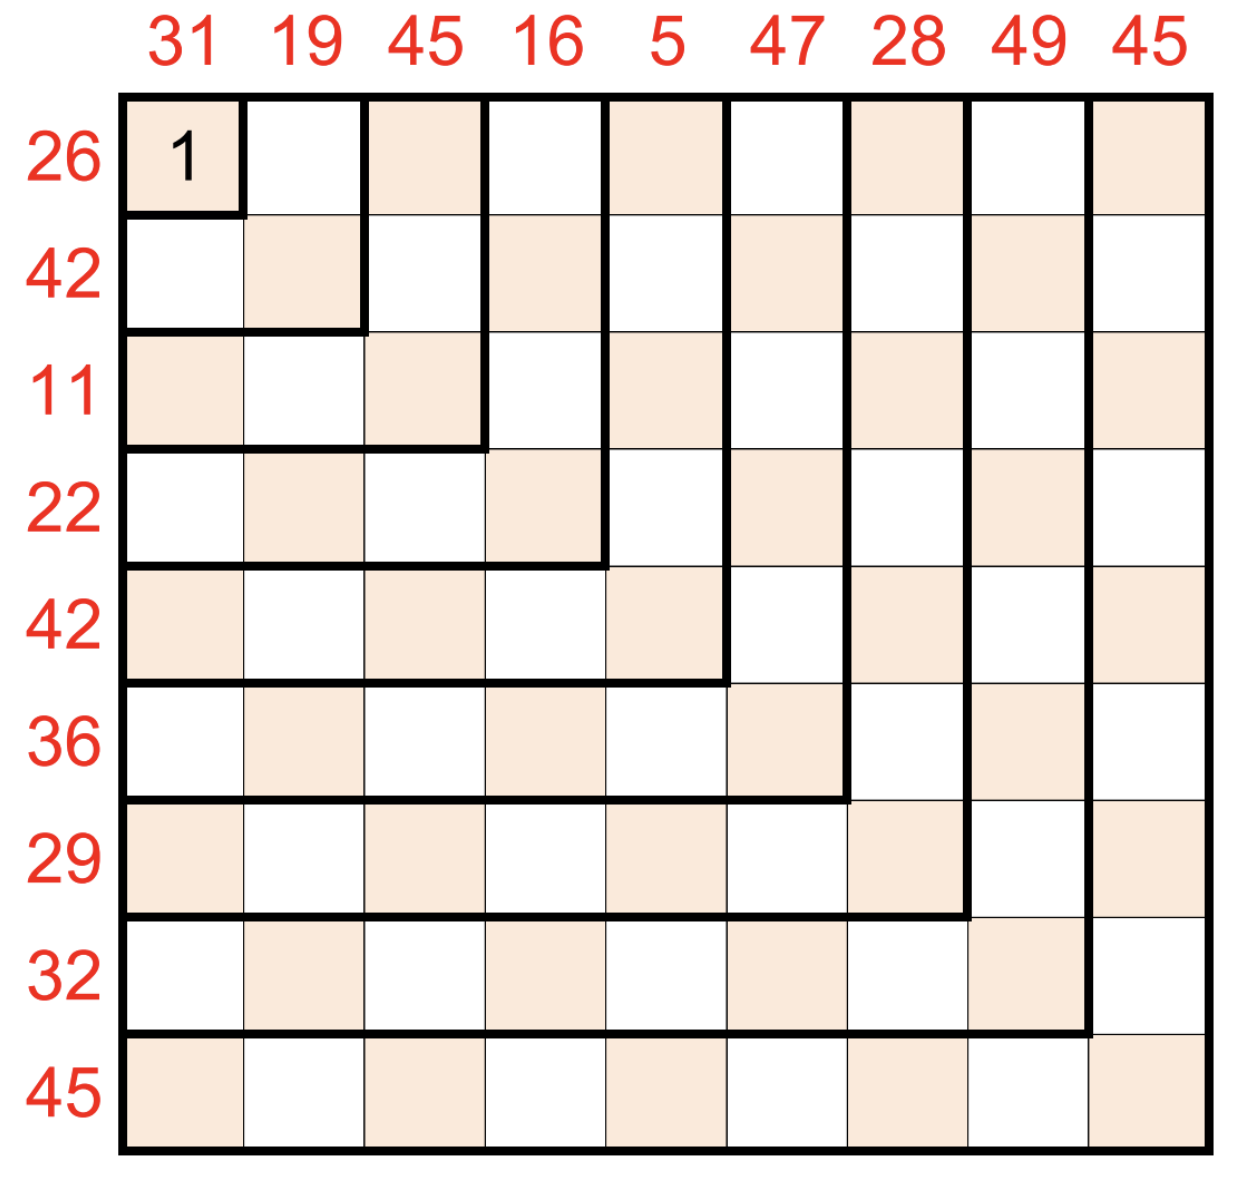
\includegraphics[scale=0.4]{puzzle1}
\end{center}
It was easy to solve given enough time because I could fill out the grid from the bottom right corner one by one. I figured that it would be easy to manipulate the answer (eg.\ add/multiply certain squares) so I can get the number I want with  puzzles similar to this.
\section*{A Counting Problem}
\textbf{09/23/2024}\\
This is a counting problem I struggled to solve without any hints. 
\begin{quote}
For $n \geq 4$, consider the strings made up of $n$ bits --- that is, a total of n 0's and 1's. In particular, consider those strings where there are (exactly) two occurrences of 01. How many such strings are there?
\end{quote}
I wrote down the small cases to find a pattern. 
\begin{center}
\begin{tabular} {|c|c|c|c|c|}
\hline
 \diagbox{$n$}{\# of 01} & \textbf{0} & \textbf{1} & \textbf{2} & \textbf{3}\\
 \hline
 \textbf{4} & 5 & 10 & 1 & 0\\
 \hline
 \textbf{5} & 6 & 20 & 6 & 0\\
 \hline
 \textbf{6} & 7 & 35 & 21 & 1\\
 \hline
 \textbf{7} & 8 & 56 & 56 & 8\\
 \hline
\end{tabular}
\end{center}
I counted the small cases with hand, and I used that the sum of the numbers in a row must add up to $2^n$ to fill the rest of the table. After completing the third row, I noticed that all the numbers in $n$th row are from $(n+1)$th row of Pascal's triangle, so I used this fact to complete the fourth row. I eventually guessed the formula for the number of binary strings of length $n$ with $k$ 01s to be $\binom{n+1}{2k+1}$. However, I could not figure out how choosing $2k+1$ out of $n+1$ objects can represent a binary string of length $n$ with $k$ 01s. I examined the specific case of $n=6$, $k=2$ and $\binom{n+1}{2k+1} = \binom{7}{5}$. I counted how many times 0 switches to 1 or 1 to 0 for the string to have 2 occurrences of 01, and there were 4 cases if I shortened any repeating digits to just one of them. \\

\begin{tabular}{c l l}
1) & 0101 & Switches 3 times\\
2) & 01010 & Switches 4 times\\
3) & 10101 & Switches 4 times\\
4) & 101010 & Switches 5 times\\
\end{tabular}\\

\noindent I realized that you can merge all four cases by putting 1 at the front and 0 at the end.\\

\begin{tabular}{c l c l}
1) & 0101 & $\rightarrow$ & 101010\\
2) & 01010 & $\rightarrow$ & 101010\\
3) & 10101 & $\rightarrow$ & 101010\\
4) & 101010 & $\rightarrow$ & 101010\\
\end{tabular}\\

\noindent With extra 1 and 0, there are now 8 letters and thus 7 places (between each letter) where 0 and 1 can be switched, and they are always switched 5 times. We now choose 5 out of 7 places to have exactly 2 occurrences of 01, so we obtain the desired number, $\binom{7}{5}$. To generalize, there are $\binom{n+1}{2k+1}$ strings with exactly $k$ occurrences of 01 and length $n$. Thus, the answer we are looking for is $\binom{n+1}{5}$.
\section*{Putnam 2013 A1}
\textbf{09/24/2024}\\
Here's another simple problem from the Putnam competition. 
\begin{quote}
Recall that a regular icosahedron is a convex polyhedron having 12 vertices and 20 faces; the faces are congruent equilateral triangles. On each face of a regular
icosahedron is written a nonnegative integer such that
the sum of all 20 integers is 39. Show that there are
two faces that share a vertex and have the same integer
written on them.
\end{quote}
When I tried this problem, I tried to figure out the maximum number of same integer that can be written by drawing out the icosahedron and trying to put in single number as many as possible. I was able to put 4 without a sharing vertex, but I wasn't able to find a way to put 5. I figured 4 was the maximum although I couldn't think of a way to prove it. To minimize the sum, I needed to put 5 smallest nonnegative integers (0, 1, 2, 3, 4) 4 times each which gives the sum of $4 \cdot (0 + 1 + 2 + 3 + 4) = 40$. Thus, the sum of 39 cannot be achieved without two faces sharing a vertex and having the same integer written on them. This solution is valid if I could prove that 4 is the maximum number of same integer that can be written.

It turned out that there was a simple and beautiful proof for it. If the same integer is written on 5 different triangular faces, and none of the vertices are shared, then there are 15 different vertices in an icosahedron. Since there are only 12 vertices in an icosahedron,  the maximum number of same integer that can be written is 4.

Asking what the minimum sum of the numbers with no two faces that share a vertex and have the same integer instead of proof questions will allow this problem to be used in Lockbox. The conditions can also be adjusted to get a number we want.
\section*{Linear Recurrences}
\textbf{09/29/2024}\\
When a term $a_n$ in a sequence $a_1, a_2, a_3, \cdots a_n, a_{n+1}, \cdots$ is defined by its preceding terms, it is a recurrence. It is a linear homogenous reccurrence of degree $k$ if the recurrence relation is in a form \[a_n = c_1a_{n-1} +  c_2a_{n-2} + c_3a_{n-3} + \cdots + c_ka_{n-k}\]  We can obtain an explicit formula for $a_n$ given the relation and the first $k$ terms of the sequence. 

First, we try to find any $a_n = x^n$ with $x \neq 0$ that satisfies the relation. 
\begin{eqnarray*}
x^n & = & c_1x^{n-1} +  c_2x^{n-2} + c_3x^{n-3} + \cdots + c_kx^{n-k}\\
x^{n-k}(x^k & = & c_1x^{k-1} +  c_2x^{k-2} + c_3x^{k-3} + \cdots + c_k)\\
x^k & = & c_1x^{k-1} +  c_2x^{k-2} + c_3x^{k-3} + \cdots + c_k \text{ since } r \neq 0\\
x^k - c_1x^{k-1} +- c_2x^{k-2} - c_3x^{k-3} - \cdots - c_k &=& 0
\end{eqnarray*}
This is called the \emph{characteristic equation}, and we can obtain the roots $x=r_i$ with  $1 \leq i \leq k$ where each $a_n = r_i^n$ satisfies the initial relation. We will first consider the case where all the roots are distinct.

If $r_1^n$ and $r_2^n$ satisfy the relation, $\alpha_1 r_1^n + \alpha_2 r_2^n$ also satisfy the relation. 
\begin{eqnarray*}
r^n & = & c_1r^{n-1} +  c_2r^{n-2} + \cdots + c_kr^{n-k}\\
\Leftrightarrow \alpha r^n & = & c_1\alpha r^{n-1} +  c_2\alpha r^{n-2} + \cdots + c_k\alpha r^{n-k}\\
(\alpha_1 r_1^n + \alpha_2 r_2^n) & = & c_1(\alpha_1 r_1^{n-1} + \alpha_2 r_2^{n-1}) +  c_2(\alpha_1 r_1^{n-2} + \alpha_2 r_2^{n-2}) + \cdots + c_k(\alpha_1 r_1^{n-k} + \alpha_2 r_2^{n-k})\\
\end{eqnarray*}
Therefore, we can combine all the $r_i^n$ to find $a_n$ that not only satisfies the relation but also matches the first $k$ terms.

Here's an example for better understanding. This is a problem from the Canadian Lynx Mathematical Competition 2023.
\begin{quote}
\textbf{\#13:} You are given a biased coin, where Heads comes up with probability $\frac{2}{3}$ and Tails comes up with probability $\frac{1}{3}$.\\\\You play a game where you start with 0 points. Each time you flip Heads, you add 2 points to your score. Each time you flip Tails, you add 1 point to your score.\\\\If you reach \emph{exactly n} points, then you win. However, if you \emph{go over n} points, then you lose.\\\\Let $P_n$ be the probability that you win the game with a target score of $n$ points.\\\\Determine the value of $P_8$.
\end{quote}
First, $P_0 = 1$ and $P_1 = \frac{1}{3}$ trivially. For $n \geq 2$, we can reach exactly $n$ points by flipping Heads with $n-2$ points or flipping Tails with $n-1$ points. This is a linear homogenous recurrence relation:\[P_n = \frac{1}{3}P_{n-1} + \frac{2}{3}P_{n-2}\] With its characteristic equation, I can find two solutions that satisfy the recurrence.
\begin{eqnarray*}
x^2 & = & \frac{1}{3}x + \frac{2}{3}\\
3x^2 & = & x + 2\\
3x^2 - x - 2 & = & 0\\
(3x+2)(x-1) & = & 0\\
x & = & -\frac{2}{3}, 1
\end{eqnarray*}
Since we know $(-\frac{2}{3})^n$ and $1^n$ satisfy the recurrence, we try to find $\alpha_1$ and $\alpha_2$ so $P_n = \alpha_1(-\frac{2}{3})^n + \alpha_2(1)^n$ matches $P_0 = 1$ and $P_1 = \frac{1}{3}$. 
\begin{align*}
&\begin{dcases}
\alpha_1\left(-\frac{2}{3}\right)^0 + \alpha_2(1)^0 & = 1\\
\alpha_1\left(-\frac{2}{3}\right)^1 + \alpha_2(1)^1 & = \frac{1}{3}\\
\end{dcases}\\\\
&\begin{dcases}
\alpha_1 + \alpha_2 & = 1\\
-\frac{2}{3}\alpha_1 + \alpha_2 & = \frac{1}{3}\\
\end{dcases}\\\\
&\begin{dcases}
\alpha_1 & = \frac{2}{5}\\
\alpha_2 & = \frac{3}{5}
\end{dcases}
\end{align*}
We find that $\displaystyle P_n = \frac{2}{5}\left(-\frac{2}{3}\right)^n + \frac{3}{5}(1)^n = \frac{2}{5}\left(-\frac{2}{3}\right)^n + \frac{3}{5}$. We can see that this is valid by substituting:
\begin{eqnarray*}
P_n & = & \frac{1}{3}P_{n-1} + \frac{2}{3}P_{n-2}\\
\frac{2}{5}\left(-\frac{2}{3}\right)^n + \frac{3}{5} & = & \frac{1}{3}[\frac{2}{5}\left(-\frac{2}{3}\right)^{n-1} + \frac{3}{5}] + \frac{2}{3}[\frac{2}{5}\left(-\frac{2}{3}\right)^{n-2} + \frac{3}{5}]\\
& = & \frac{2}{15}\left(-\frac{2}{3}\right)^{n-1} + \frac{1}{5} + \frac{4}{15}\left(-\frac{2}{3}\right)^{n-2} + \frac{2}{5}\\
& = & \frac{2}{15}\left(-\frac{2}{3}\right)^{-1}\left(-\frac{2}{3}\right)^n + \frac{1}{5} + \frac{4}{15}\left(-\frac{2}{3}\right)^{-2}\left(-\frac{2}{3}\right)^n + \frac{2}{5}\\
& = & -\frac{1}{5}\left(-\frac{2}{3}\right)^n + \frac{1}{5} + \frac{3}{5}\left(-\frac{2}{3}\right)^n + \frac{2}{5}\\
& = & \frac{2}{5}\left(-\frac{2}{3}\right)^n + \frac{3}{5}
\end{eqnarray*}
Thus, $\displaystyle P_8 = \frac{2}{5}\left(-\frac{2}{3}\right)^8 + \frac{3}{5} = \frac{4039}{6561}$.

Like this example, given numeric values of two terms ($P_{m_1} = c_1, P_{m_2} = c_2$ where $m_1 \neq m_2$) and a linear homogenous recurrence of degree 2 with its characteristic equation having 2 distinct roots $r_1$ and $r_2$, we can always find the explicit formula for the general term $a_n$. It is equivalent to finding a solution to this system of equations with two equations and two unknown variables, $\alpha_1$ and $\alpha_2$.
\[
\begin{cases}
\alpha_1 r_1^{m_1} + \alpha_2 r_2^{m_1} = c_1\\
\alpha_1 r_1^{m_2} + \alpha_2 r_2^{m_2} = c_2
\end{cases}
\]
This always has a solution if two slopes of each equation drawn on a plane are different. In a slope-intercept form ($\alpha_1$ as $x$ and $\alpha_2$ as $y$):
\[
\begin{dcases}
\alpha_2 = -\left(\frac{r_1}{r_2}\right)^{m_1}\alpha_1 + \frac{c_1}{r_2^{m_1}}\\
\alpha_2 = -\left(\frac{r_1}{r_2}\right)^{m_2}\alpha_1 + \frac{c_2}{r_2^{m_2}}\\
\end{dcases}
\]
The slopes are: $\displaystyle -\left(\frac{r_1}{r_2}\right)^{m_1}, -\left(\frac{r_1}{r_2}\right)^{m_2}$, which must be different since $r_1 \neq r_2$ and $m_1 \neq m_2$. Therefore, we can always find $a_1$ and $a_2$ and thus the explicit formula for $a_n$. This generalizes to linear homogenous recurrences of higher degrees where all the roots of their characteristc equations are distinct.

Now, let's consider the case where some of the roots are identical. If the characteristic equation $x^2 - c_1x - c_2 = 0$ of $a_n = c_1a_{n-1} + c_2a_{n-2}$ has a double root $r$, then $nr^n$ as well as $r^n$ satisfies the recurrence. This is because $r$ is also a root of the derivative of the characteristic equation:
\begin{eqnarray*}
a_n &=& c_1a_{n-1} + c_2a_{n-2}\\
nx^n &=& c_1(n-1)x^{n-1} + c_2(n-2)x^{n-2}\\
nx^n - c_1(n-1)x^{n-1} - c_2(n-2)x^{n-2} &=& 0\\
x(nx^{n-1} - c_1(n-1)x^{n-2} - c_2(n-2)x^{n-3} &=& 0\\
x \cdot \frac{d}{dx}\left(x^n - c_1x^{n-1} - c_2x^{n-2}\right) &=& 0\\
x \cdot \frac{d}{dx}\left(x^{n-2}(x-r)^2\right) &=& 0\\
x [(n-2)x^{n-3}(x-r)^2 + x^{n-2}\cdot 2(x-r)] &=& 0\\
x^{n-2}(x-r)[(n-2)(x-r) + 2x)] &=& 0\\
\therefore x \text{ can be } r \text{, and } nr^n \text{satisfies the recurrence.}
\end{eqnarray*}
By similar reasoning, if a root of a characteristic equation $r$ has a multiplicity of $k$, then $\displaystyle \frac{n!}{(n-i+1)!} \cdot r^n$ for $1 \leq i \leq k$ satisfy the recurrence relation. Then the general form includes $\alpha_1 r^n + \alpha_2 nr^n + \alpha_3 n(n-1)r^n + \cdots \alpha_k\frac{n!}{(n-i+1)!}r^n$ which can be written as $\alpha_1 r^n + \alpha_2 nr^n + \alpha_3 n^2r^n + \cdots \alpha_kn^kr^n$ since $\alpha_i$'s are variables. Now, we can find the explicit formula for the general term of any linear homogenous recurrence relationships.

To summarize, given a linear homogenous recurrence relationship in form
\[a_n = c_1a_{n-1} +  c_2a_{n-2} + c_3a_{n-3} + \cdots + c_ka_{n-k},\]
and $k$ terms, first find the roots of its characteristic equation,
\[x^k - c_1x^{k-1} - c_2x^{k-2} - c_3x^{k-3} - \cdots - c_k = 0.\]
For each root $r$, if it has a multiplicity of $m$, then $n^ir^n$ for $0 \leq i \leq m - 1$ satisfy the recurrence relation. We can find $k$ terms in total, then we obtain find the explicit formula for general term $a_n$ composed of each of those $k$ terms multiplied by an unknown constant. We find the value of each constant by solving a system of equations acquired from substituting the given $k$ terms into $a_n$.
\section*{Sudoku Variant}
\textbf{10/01/2024}\\
I finally solved this variant of sudoku I found from this \href{https://www.youtube.com/watch?v=u0FhERdlWFc}{video}. The grid is on the left, and the rule is written on the right.
\begin{center}
\addtolength{\leftskip} {-2cm} % increase (absolute) value if needed
\addtolength{\rightskip}{-2cm}
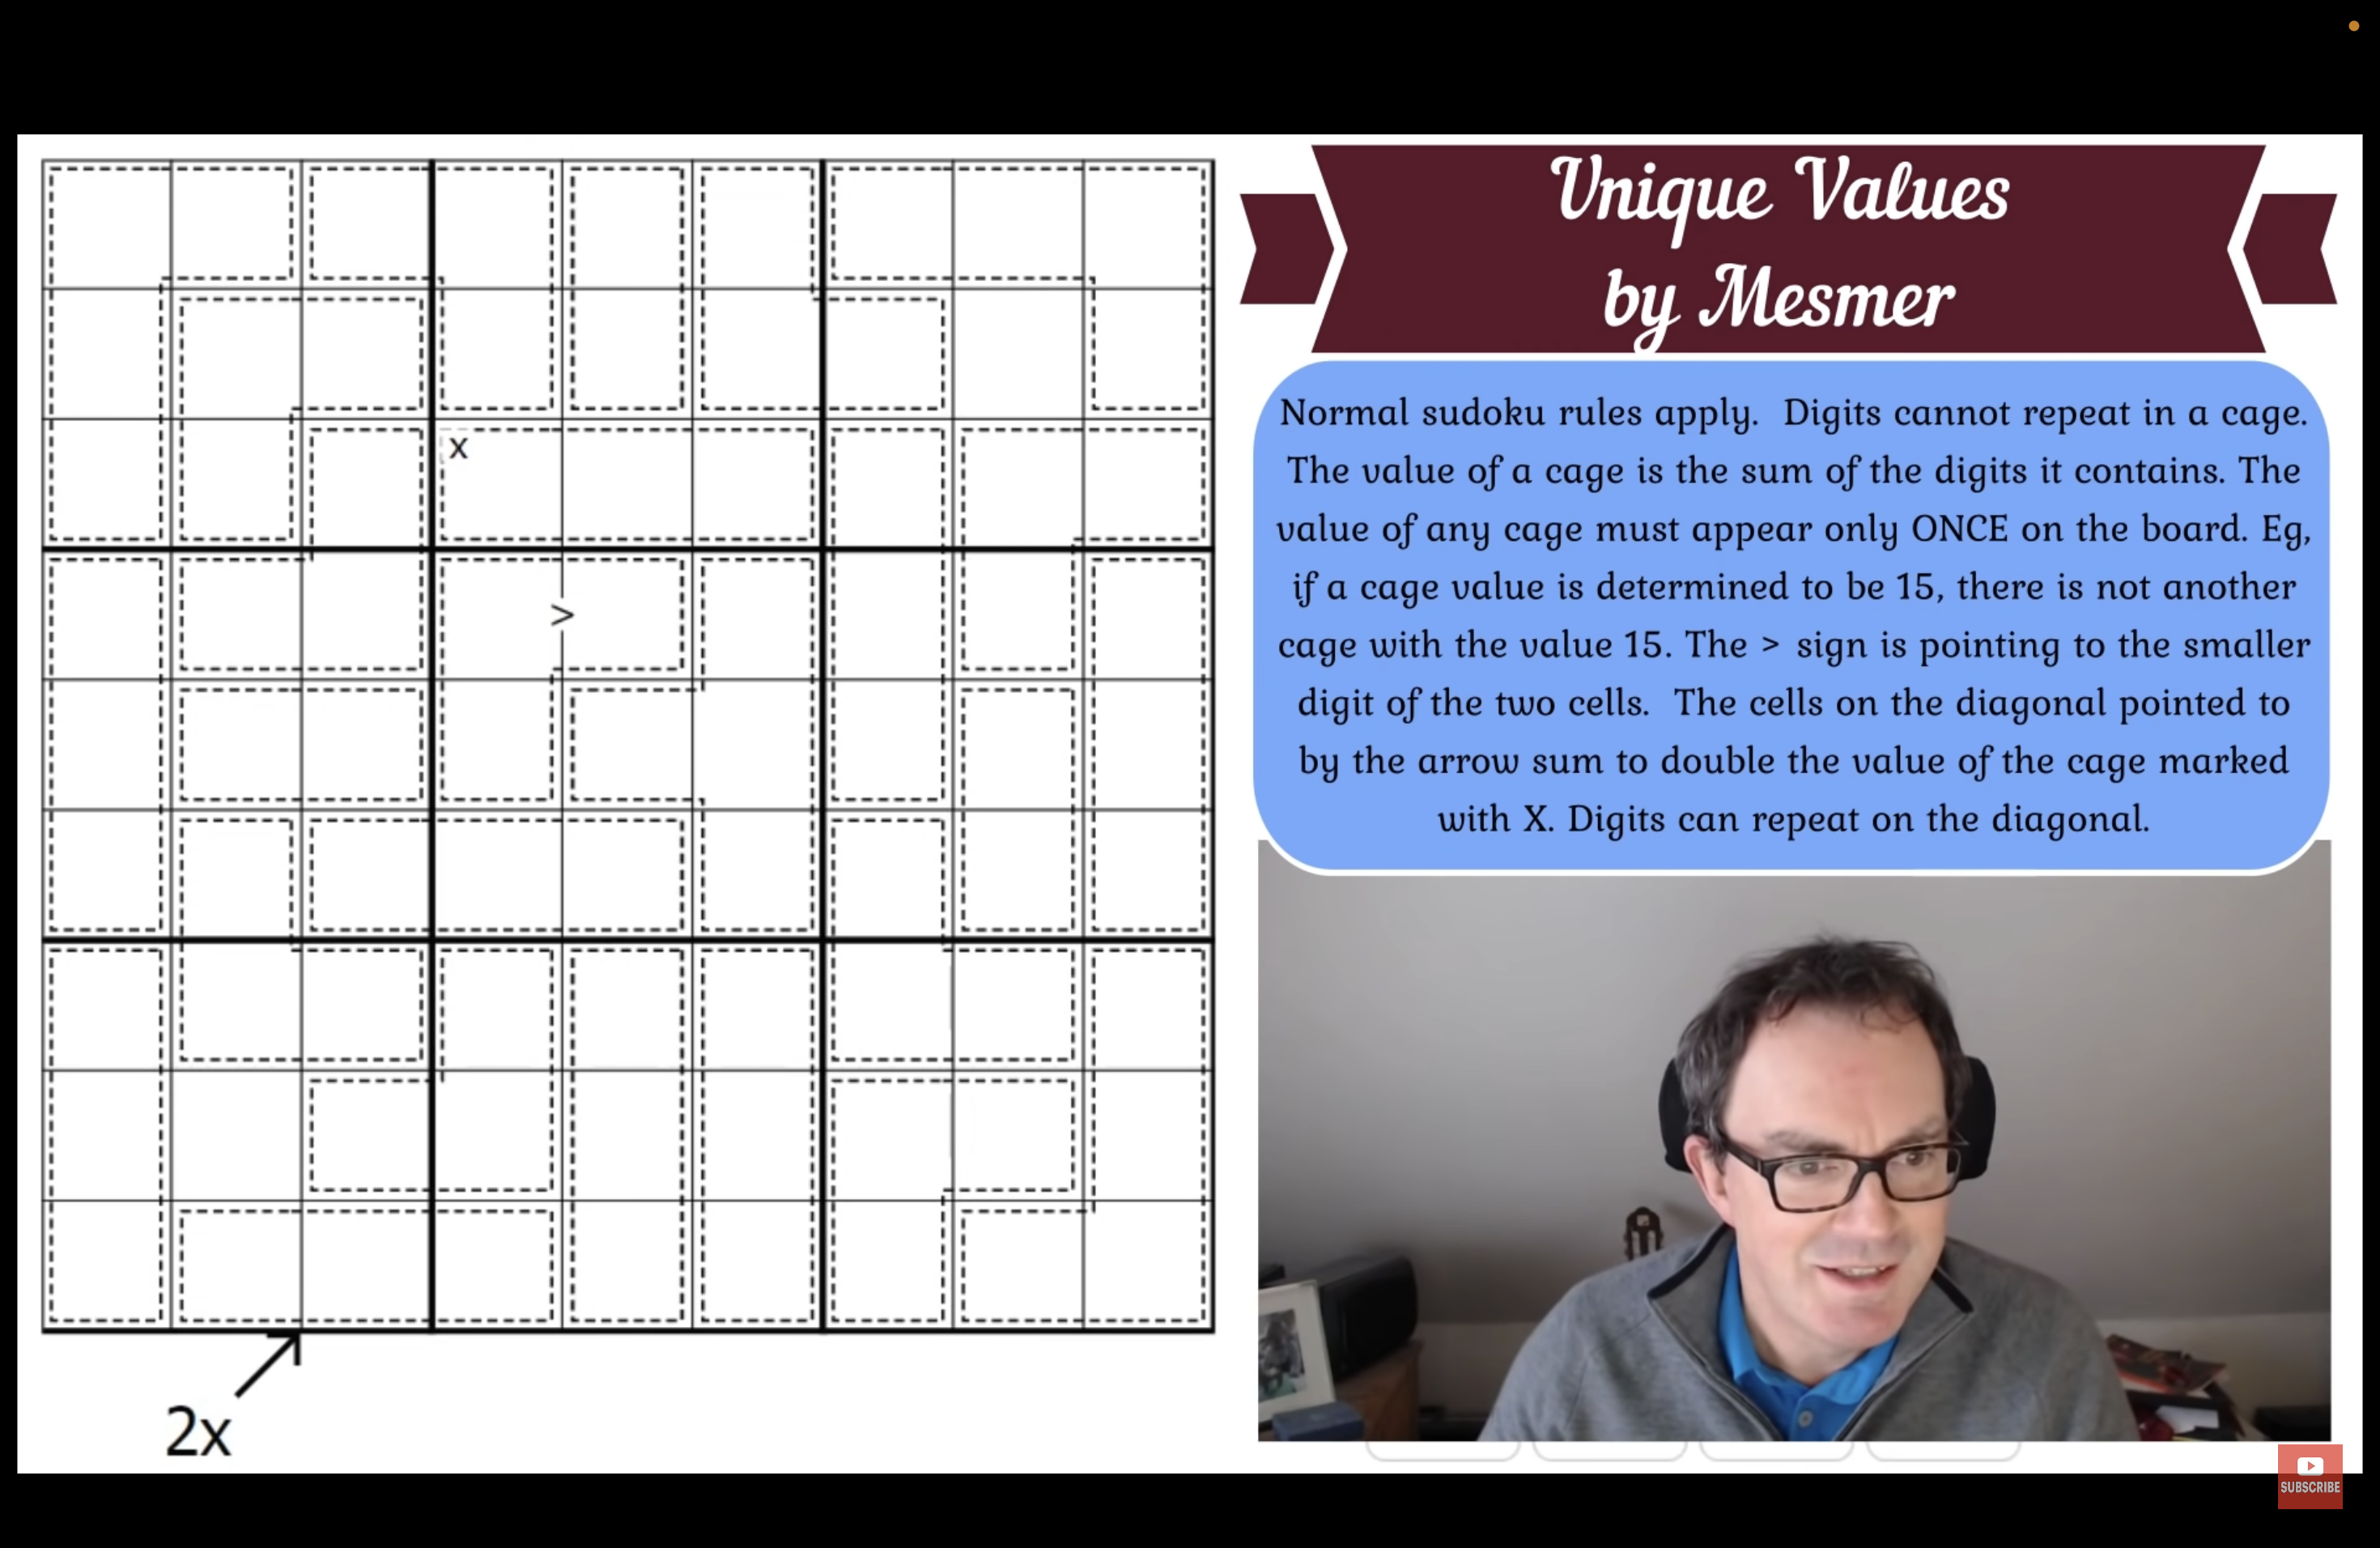
\includegraphics[scale=0.35]{puzzle2}
\end{center}
There are 3 cages of 2 cells, 19 cages of 3 cells, and 4 cages of 4 cells. The range of possible values are:
\begin{center}
\begin{tabular} {|c|c|c|}
\hline
\# of Cells & Minimum Value & Maximum Value\\
\hline
2 & $1+2=3$ & $8+9=17$\\
\hline
3 & $1+2+3=6$ & $7+8+9=24$\\
\hline
4 & $1+2+3+4=10$ & $6+7+8+9=30$\\
\hline
\end{tabular}
\end{center}
There are 19 possible values for 19 cages of 3 cells, so every single value must be used. Then, after excluding 6 to 24 from the range of values of cages of 2 cells, there are 3 possible values for 3 cages of 2 cells, so all of these must be used, too. Now the minimum value of the sum of all cages is sum of all integers from 3 to 28 which is $\frac{(3+28)(28-3+1)}{2} = 403$ when there are two cells in the entire grid that is not caged, and the sum of all numbers in a grid must be $\frac{9(1+9)}{2}\cdot9 = 405$. The sum of uncaged two cells cannot be less than 2, so the value of 4 cages of 4 cells must be 25 to 28 while the two uncaged cells are both 1. From here, I just eliminated possibilities and filled out the determined digits one by one until it was finished. Here's the completed version:
\begin{center}
\addtolength{\leftskip} {-2cm} % increase (absolute) value if needed
\addtolength{\rightskip}{-2cm}
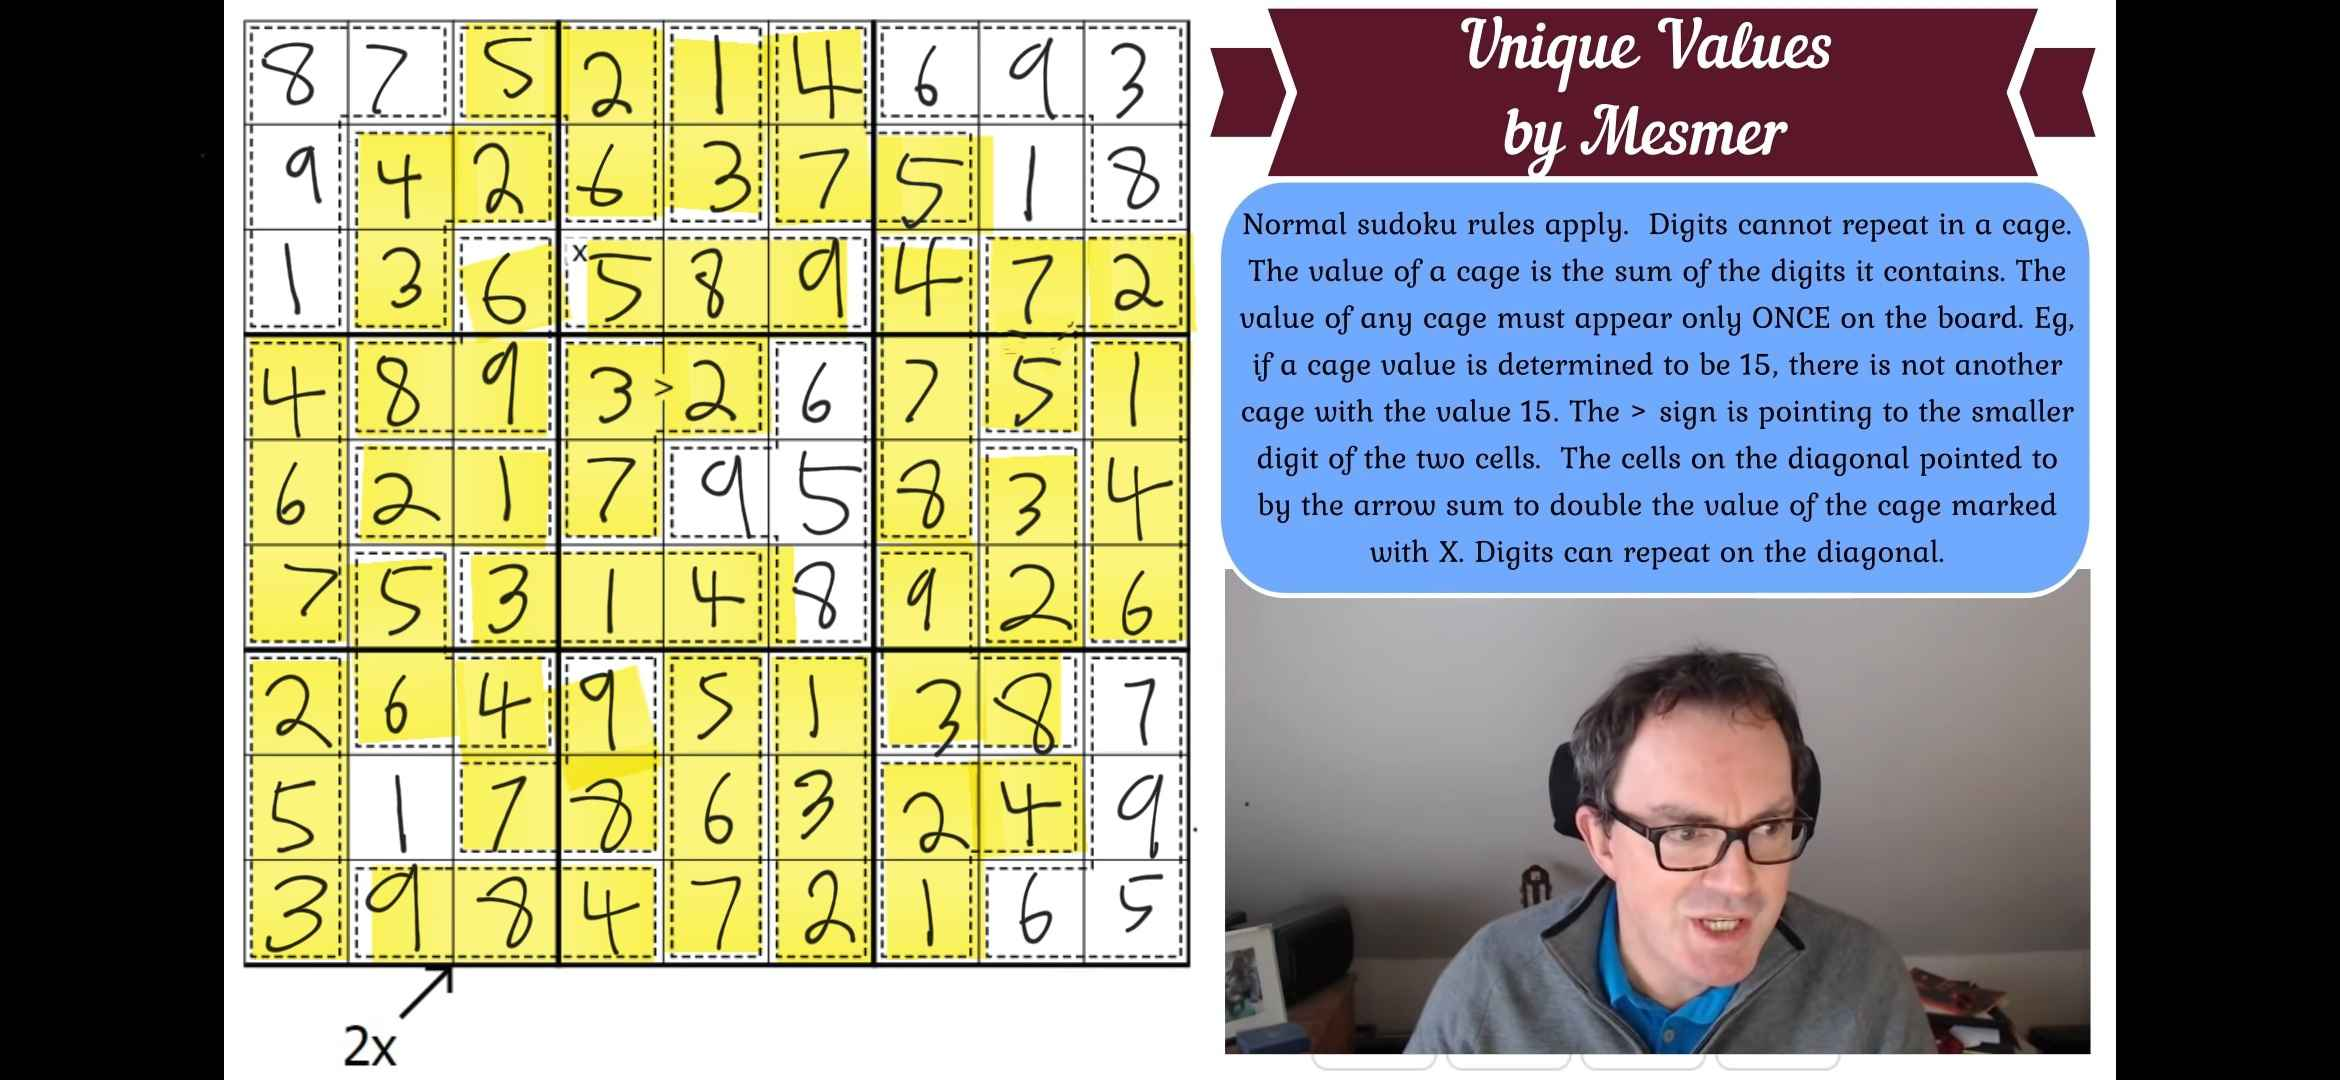
\includegraphics[scale=0.22]{puzzle2sln}
\end{center}
I have solved a total of three variants of sudoku introduced by the same YouTube channel, and they were all really fun. I will keep trying the fun-looking ones when I have spare time.
\section*{$\frac{\pi}{n} \sim \sin(\frac{\pi}{n})$}
\textbf{10/02/2024}\\
In an introductory assignment to Python turtle graphics, a drawing tool, I first made a function that draws a regular polygon with $n$ sides with each side length $l$. Then, I was told to make a function that draws a circle using the polygon function to draw a regular polygon with a lot of sides. However, I was only given a radius $r$ when I needed the length of each sides. I figured dividing the circumference of a circle by the number of sides will give me the length of each side, giving me this formula: \[l = 2 \cdot r \cdot \pi / n.\] However, the instruction told me to use this formula: \[l = 2 \cdot r \cdot \sin(\pi / n).\] I eventually figured out how to derive this formula.
\begin{center}
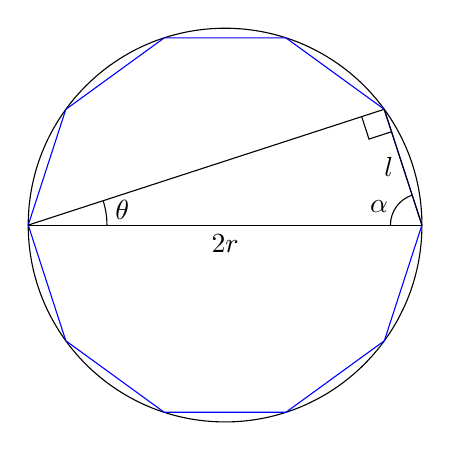
\begin{tikzpicture}
\draw circle(2.5cm);
\coordinate (A) at (-2.5,0);
\coordinate (B) at (2.5,0);
\coordinate (C) at (2.02,1.47);
\node[blue, regular polygon, regular polygon sides=10, minimum size=5cm, draw] {};
\draw (A) -- (B) node[below, midway]{$2r$};
\draw (A) -- (C);
\draw (B) -- (C) node[left, midway, shift={(0mm,0mm)}]{$l$};
\draw pic[draw,angle radius=1cm,"$\theta$" shift={(6mm,1mm)}] {angle=B--A--C};
\draw pic[draw,angle radius=4mm,"$\alpha$" shift={(-3.5mm,1mm)}] {angle=C--B--A};
\draw pic[draw,angle radius=3mm] {right angle=A--C--B};
\end{tikzpicture}
\end{center}
Draw a right triangle with its hypotenuse the diameter of the circle and one side being the side of the regular polygon. The angle opposed to the side $\theta$ is $\dfrac{\pi}{n}$.
\begin{eqnarray*}
\theta & = & \frac{\pi}{2} - \alpha\\
& = & \frac{\pi}{2} - \frac{1}{2} \cdot \text{(interior angle of regular polygon)}\\
& = & \frac{\pi}{2} - \frac{1}{2} \cdot \frac{\pi \cdot n - 2 \cdot \pi}{n}\\
& = & \frac{\pi}{n}\\
\end{eqnarray*}
From this, 
\begin{eqnarray*}
& \sin(\pi/n) = \dfrac{l}{2r}\\
\Leftrightarrow & l = 2 \cdot r \cdot \sin(\pi/n).
\end{eqnarray*}
Here, I couldn't find any flaw in logic for both formulas, so I wondered if $\sin(\pi/n)$ and $\pi/n$ were equal. However, I knew that cannot be the case, then I realized this is a special case where $n$ is supposed to be as big as possible. $\sin\left(\dfrac{\pi}{n}\right) = \dfrac{\pi}{n}$ holds true when $n$ approaches infinity. If $\sin\left(\dfrac{\pi}{n}\right) = \dfrac{\pi}{n}$, then $\dfrac{\sin\left(\dfrac{\pi}{n}\right)}{\dfrac{\pi}{n}} = 1$. We can write:
\[\lim_{n\rightarrow\infty} \dfrac{\sin\left(\dfrac{\pi}{n}\right)}{\dfrac{\pi}{n}} = 1\] 
Substitute $x = \dfrac{\pi}{n}$ which approaches 0 as $n$ approaches $\infty$.\\
\[\lim_{x\rightarrow0} \dfrac{\sin(x)}{x} = 1\]
Now, this was a familiar limit I had learned previously. It was cool to see how this limit can be shown geometrically.
\section*{Sum of Divisiors}
\textbf{10/04/2024}\\
\begin{quote}If sum of the divisors of $n$ (including $n$) is greater than $4n$, what is the lowest number of $n$'s prime divisors?\end{quote}
Write $n = p_1^{e_1}p_2^{e_2} \cdots p_k^{e_k}$ with each $p_i$ being a distinct prime factor of $n$. Say $S(n)$ represent the sum of all divisors of $n$, then \[S(n) = \left(\frac{p_1^{e_1+1}-1}{p_1-1}\right)\left(\frac{p_2^{e_2+1}-1}{p_2-1}\right)\cdots\left(\frac{p_k^{e_k+1}-1}{p_k-1}\right).\] Since $S(n) > 4n$, it follows that $\dfrac{S(n)}{n} > 4$.
\begin{eqnarray*}
\dfrac{S(n)}{n} & = & \dfrac{\left(\dfrac{p_1^{e_1+1}-1}{p_1-1}\right)\left(\dfrac{p_2^{e_2+1}-1}{p_2-1}\right)\cdots\left(\dfrac{p_k^{e_k+1}-1}{p_k-1}\right)}{p_1^{e_1}p_2^{e_2} \cdots p_k^{e_k}}\\
& = & \left(\frac{p_1^{e_1+1}-1}{p_1^{e_1}(p_1-1)}\right)\left(\frac{p_2^{e_2+1}-1}{p_2^{e_2}(p_2-1)}\right)\cdots\left(\frac{p_k^{e_k+1}-1}{p_k^{e_k}(p_k-1)}\right)\\
& = & \left(\dfrac{p_1-\dfrac{1}{p_1^{e_1}}}{p_1-1}\right)\left(\dfrac{p_2-\dfrac{1}{p_2^{e_2}}}{p_2-1}\right)\cdots\left(\dfrac{p_k-\dfrac{1}{p_k^{e_k}}}{p_k-1}\right)\\
\end{eqnarray*}
We can maximize the exponent of each prime factor to maximize $\dfrac{S(n)}{n}$:
\[
\left(\dfrac{p_1-\dfrac{1}{p_1^{e_1}}}{p_1-1}\right)\left(\dfrac{p_2-\dfrac{1}{p_2^{e_2}}}{p_2-1}\right)\cdots\left(\dfrac{p_k-\dfrac{1}{p_k^{e_k}}}{p_k-1}\right) < \left(\dfrac{p_1}{p_1-1}\right)\left(\dfrac{p_2}{p_2-1}\right)\cdots\left(\dfrac{p_k}{p_k-1}\right)
\]
The left side can be arbitrarily close to the right side since maximizing the exponents will cause $\dfrac{1}{p_i^{e_i}}$ to approach 0. Notice that $\dfrac{p_i}{p_i-1}$ decreases as $p_i$ increases, so we want each prime factor to be as small as possible. If the lowest number of $n$'s prime divisors is 3, then $S(n)/n$ is maximized when the prime divisors are 2, 3 and 5:
\[
\frac{S(n)}{n} < \frac{2}{1} \cdot \frac{3}{2} \cdot \frac{5}{4} = \frac{15}{4} < 4
\]
$S(n)/n$ can never reach 4. If the lowest number of $n$'s prime divisors is 4, then $S(n)/n$ is maximized when the prime divisors are 2, 3, 5 and 7:
\[
\frac{S(n)}{n} < \frac{2}{1} \cdot \frac{3}{2} \cdot \frac{5}{4} \cdot \frac{7}{6} = \frac{35}{8} > 4
\]
This means $S(n)/n$ can get arbitrarily close to $\dfrac{35}{8}$, which is bigger than 4. Thus, the lowest number of $n$'s prime divisors for the sum of the divisors of $n$ to be greater than $4n$ is 4.
\end{document}